\documentclass{article}
\input{../preamble}
\usepackage{cancel}
\input{unit4glossary}


\usepackage{fancyhdr}
\pagestyle{fancy}
\renewcommand{\headrulewidth}{0pt}
\renewcommand{\headruleskip}{0mm}
\fancyfoot[C]{Access for free at \href{https://openstax.org/books/physics/pages/1-introduction}{https://openstax.org/books/physics/pages/1-introduction}
\hfill \thepage}
\fancyhead{}
    
\newif\iflong %boolean
\longfalse %change to \longtrue (\longfalse) to show (hide) solutions.

\numberwithin{equation}{section}
\setcounter{section}{4}
\numberwithin{figure}{section}

\makenoidxglossaries 



\title{Unit 4: Forces}
\author{Edited by Luis Nunez}
\date{Updated on \today}


\begin{document}
\maketitle

% Physics \hfill Unit 4: Forces \hfill Lecture Notes
% \vspace{-0.8em}

% \hfill {\footnotesize Updated: \today}

% \framebox{\textbf{Link}} \textit{YouTube}: ``Breaking Bad: Destroying the Evidence'' by \texttt{SonyPicturesDVD} (\href{https://youtu.be/gzCXowhks80?t=3}{click here}). An example of the magnetic force.

% \framebox{\textbf{Link}} \textit{YouTube}: ``Jumping From Space! Red Bull Space Dive'' by \texttt{BBC Studios} (\href{https://youtu.be/E9oKEJ1pXPw}{click here}) An example of the gravitational force.

% \framebox{\textbf{Link}} \textit{PhET Simulation}: ``Forces and Motion: Basics'' (\href{https://phet.colorado.edu/en/simulations/forces-and-motion-basics}{click here}).


\subsection{Newton's First Law of Motion} \label{XeoZti}

A \gls{force} is a push or a pull. Examples of a force include pushing a car to get it moving, the \href{https://youtu.be/gzCXowhks80?t=3}{magnetic force}, and the \href{https://youtu.be/E9oKEJ1pXPw}{gravitational force}. Force is a vector: it's represented by an arrow with a direction and a magnitude that is measured in units of newtons (N). Forces act on an object or system. 

\begin{mdframed}[backgroundcolor=black!10]
\gls{NIL} is summarized in 3 facts:
\vspace{-1ex}

\begin{enumerate}
\setlength\itemsep{0ex}
    \item An object at rest stays at rest.
    \item An object in motion stays in motion in a straight line at a constant speed.
    \item Facts 1 and 2 above cease being true when the object is acted upon by a net (unbalanced) force.
\end{enumerate}
\end{mdframed}

Fact 1 is obvious. Fact 2 is rarely observable on Earth, because of net forces stated in Fact 3, but it's exemplified by an asteroid or the \href{https://voyager.jpl.nasa.gov/mission/status/}{Voyager spacecrafts}. When addressing Newton's laws of motion, we may need to refer to the mass or inertia of the object. \Gls{mass} is the amount of matter in an object. It's measured in kilograms (kg). 1 kilogram is about 2.2 pounds. \Gls{inertia} is the tendency of an object to remain at rest or in motion. For example, once released, a bowling ball will tend to stay in motion. There are many examples of inertia in sports, as when players fall by their overwhelming tendency to stay in motion; see \href{https://youtu.be/5PKXs8i_zSw?t=21}{soccer}, \href{https://youtu.be/4TgpW0WZZ6U?t=55}{football}, and \href{https://youtu.be/IGBpvIXGMYQ?t=26}{basketball}. Inertia is proportional to the object's mass: if mass increases, inertia increases.

\begin{example}
Two objects---an airplane and a person---travel on a runway each at a speed of 3 meters per second. Which object has more inertia?
\end{example}

\Solution Inertia is proportional to mass. The airplane, with its vastly greater mass, has more inertia. Furthermore, it's easy to stop a person in their tracks; good luck trying to stop a \SI{400000}{lbs.} Boeing 747.
\vspace{2ex}
\cyanhrule

\subsection*{\ref{XeoZti} Exercises}


\begin{exercise} \label{prob:fgm}
In your own words summarize Newton's First Law of Motion. Given some examples of each fact of the First Law. 
\end{exercise}


\begin{exercise} \label{WTFwXI}
According to Fact 2 of Newton's First Law, it's expected that when you let go of a shopping cart it will continue traveling at a constant speed in one direction forever. From experience, however, we know that the shopping cart always comes to a stop. (a) Does this observation violate Newton's First Law of Motion? (b) What causes the shopping cart to come to rest? (\textit{Hint}: See Fact 3.)
\end{exercise}

\begin{exercise} \label{MB3Xar}
If you’re ever being chased by a bear, it’s recommended that you run in zig-zags rather than in a straight line. A zig-zag motion decreases the probability that the bear will catch you. (a) How does the inertia of the bear compare to yours? (b) How does the concept of inertia explain the recommendation stated above? (\textit{Hint}: Refer to Newton's First Law of Motion.)
\end{exercise}
\cyanhrule

\clearpage
\subsection{Free-body Diagrams} \label{SdNOfY}

A \gls{free-body diagram} shows all forces acting on an object. The object is a dot ($\bullet$) and the forces are vectors (arrows). When more than one force acts on an object, the \gls{net force} ($F_{\text{net}}$) is the sum of all forces. 

\begin{mdframed}[backgroundcolor=black!10]
\textit{Right Minus Left Rule}. In a free-body diagram, net force is rightward force(s) minus leftward force(s).

\begin{center}
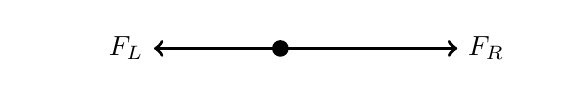
\begin{tikzpicture}
\pgfplotsset{compat=1.11}
    \begin{axis}[
        width=8cm, height=2cm,
        axis line style={draw=none},
        ticks=none,
        axis lines=middle,
        ymin=-1, ymax=1,
        xmin=-1, xmax=1,
        clip=false,
    ]
    \fill (0,0) circle (3pt);
    \draw[very thick,black,->] (0.05,0) -- (-0.5,0) node[left] {$F_{\text{L}}$};
    \draw[very thick,black,->] (-0.05,0) -- (+0.70,0) node[right] {$F_{\text{R}}$};
    % \node[right] at (1.3,0) {$F_{\text{net}} = F_{\text{R}} - F_{\text{L}}$};
    \end{axis}
\end{tikzpicture}
\end{center}
\vspace{-1em}

\begin{equation}
    \vec{F}_{\text{net}} = F_{\text{R}} - F_{\text{L}}
\end{equation}
\end{mdframed}

% Net force is calculated from a free-body diagram, as shown in the examples below. In a free-body diagram, the directions \textit{right} and \textit{up} are positive ($+$), and directions \textit{left} and \textit{down} are negative ($-$).

\begin{example} \label{ex:FnetFromFBD} 
    Two teams play tug-of-war. Team Red pushes right on a cart with a force of \SI{70}{newtons}. Team Blue applies a \SI{50}{N} leftward force. Draw a free-body diagram and calculate the net force on the cart.
\end{example}

\Solution

\begin{figure}[h!]
    \centering
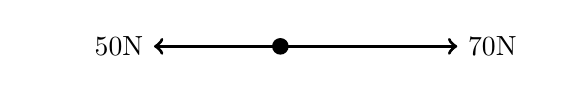
\begin{tikzpicture}
\pgfplotsset{compat=1.11}
\def\s{1}
    \begin{axis}[
        width=8cm, height=2cm,
        axis line style={draw=none},
        ticks=none,
        axis lines=middle,
        ymin=-\s, ymax=\s,
        xmin=-\s, xmax=\s,
        clip=false,
    ]
    \fill (0,0) circle (3pt);
    \draw[very thick,black,->] (0.05,0) -- (-0.5,0) node[left] {\SI{50}{N}};
    \draw[very thick,black,->] (-0.05,0) -- (+0.70,0) node[right] {\SI{70}{N}};
    \end{axis}
\end{tikzpicture}
\end{figure}

Net force is rightward force \textit{minus} leftward force:

\begin{equation*}
    \vec{F}_{\text{net}} = 70 - 50 = +\SI{20}{N}\ .
\end{equation*}

Therefore, the \textit{net} force will be to the right with a magnitude of \SI{20}{N}.

\begin{example}
\href{https://youtu.be/7e3XhWMHolU}{Spongebob and Patrick} each apply a 50-newton rightward force on a treasure chest. Mr.~Krabs applies a \SI{75}{N} leftward force. (a) Draw a free-body diagram of the chest. (b) Calculate the net force on it.
\end{example}

\Solution (a) The free-body diagram is

\begin{figure}[h!]
    \centering
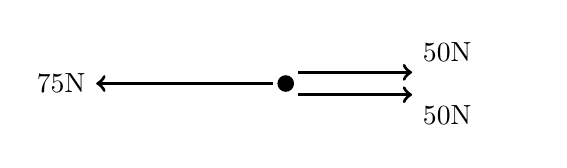
\begin{tikzpicture}
\pgfplotsset{compat=1.11}
\def\s{100} %scale
\def\FR{50} %rightward force
\def\FL{75} %leftward force
    \begin{axis}[
        width=8cm, height=3cm,
        axis line style={draw=none},
        ticks=none,
        axis lines=middle,
        ymin=-\s, ymax=\s,
        xmin=-\s, xmax=\s,
        clip=false,
    ]
    \fill (0,0) circle (3pt);
    \draw[very thick,black,->] (5,20) -- (\FR,20) node[above right] {\SI{\FR}{N}};
    \draw[very thick,black,->] (5,-20) -- (\FR,-20) node[below right] {\SI{\FR}{N}};
    \draw[very thick,black,->] (-5,0) -- (-\FL,0) node[left] {\SI{\FL}{N}};
    \end{axis}
\end{tikzpicture}
\end{figure}

(b) Net force is the sum of all forces. Computing rightward minus leftward forces leads to
\vspace{-1em}

\begin{equation*}
    \vec{F}_{\text{net}} = 50 + 50 - 75 = +\SI{25}{N}\ .
\end{equation*}

\cyanhrule

\subsection*{\ref{SdNOfY} Exercises}

\begin{multicols}{2}
\begin{exercise} \label{RApeJt}
A leftward force of \SI{50}{N} and a rightward force of \SI{150}{N} are exerted on a cart. Draw a free body diagram. What is the net force?
\end{exercise}

\begin{exercise} \label{MUJe54}
A leftward force of \SI{200}{N} and a rightward force of \SI{150}{N} are exerted on a cart. What is the net force? 
\end{exercise}

\begin{exercise} \label{Uhrg0I}
A leftward force of \SI{200}{N} and a rightward force of \SI{200}{N} are exerted on a cart. What is the net force? 
\end{exercise}

\cyanhrule
\vspace{2ex}

\columnbreak

\ref{Wu1JXi}--\ref{Js7KjP} Calculate the net force.

\begin{exercise} \label{Wu1JXi}
\phantom{.}
\vspace{-2em}
\end{exercise}

\begin{center}
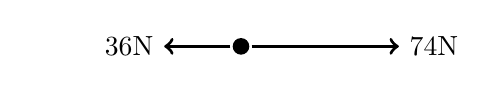
\begin{tikzpicture}
\pgfplotsset{compat=1.11}
\def\s{100} %scale
\def\FR{74} %rightward force
\def\FL{36} %leftward force
    \begin{axis}[
        width=7cm, height=2cm,
        axis line style={draw=none},
        ticks=none,
        axis lines=middle,
        ymin=-\s, ymax=\s,
        xmin=-\s, xmax=\s,
        clip=false,
    ]
    \fill (0,0) circle (3pt);
    \draw[very thick,black,->] (5,0) -- (\FR,0) node[right] {\SI{\FR}{N}};
    \draw[very thick,black,->] (-5,0) -- (-\FL,0) node[left] {\SI{\FL}{N}};
    \end{axis}
\end{tikzpicture}
\end{center}


\begin{exercise} \label{Tj5icu}
\phantom{.}
\vspace{-1cm}
\end{exercise}

\begin{center}
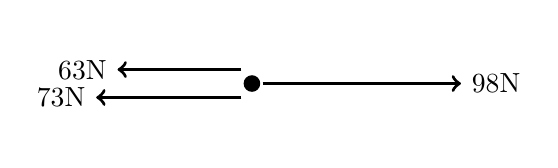
\begin{tikzpicture}
\pgfplotsset{compat=1.11}
\def\s{100} %scale
\def\FR{98} %rightward force
\def\FL{63} %leftward force
\def\FLL{73}
    \begin{axis}[
        width=7cm, height=3cm,
        axis line style={draw=none},
        ticks=none,
        axis lines=middle,
        ymin=-\s, ymax=\s,
        xmin=-\s, xmax=\s,
        clip=false,
    ]
    \fill (0,0) circle (3pt);
    \draw[very thick,black,->] (5,0) -- (\FR,0) node[right] {\SI{\FR}{N}};
    \draw[very thick,black,->] (-5,25) -- (-\FL,25) node[left] {\SI{\FL}{N}};
    \draw[very thick,black,->] (-5,-25) -- (-\FLL,-25) node[left] {\SI{\FLL}{N}};
    \end{axis}
\end{tikzpicture}
\end{center}

\begin{exercise} \label{nMwKjy}
\phantom{.}
\vspace{-3em}
\end{exercise}

\begin{center}
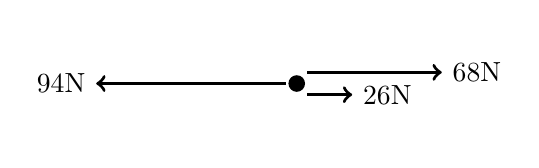
\begin{tikzpicture}
\pgfplotsset{compat=1.11}
\def\s{100} %scale
\def\FR{68} %rightward force
\def\FL{94} %leftward force
\def\FRR{26}
    \begin{axis}[
        width=7cm, height=3cm,
        axis line style={draw=none},
        ticks=none,
        axis lines=middle,
        ymin=-\s, ymax=\s,
        xmin=-\s, xmax=\s,
        clip=false,
    ]
    \fill (0,0) circle (3pt);
    \draw[very thick,black,->] (5,20) -- (\FR,20) node[right] {\SI{\FR}{N}};
    \draw[very thick,black,->] (5,-20) -- (\FRR,-20) node[right] {\SI{\FRR}{N}};
    \draw[very thick,black,->] (-5,0) -- (-\FL,0) node[left] {\SI{\FL}{N}};
    \end{axis}
\end{tikzpicture}
\end{center}


\begin{exercise} \label{Js7KjP}
\phantom{.}
\vspace{-3em}
\end{exercise}

\begin{center}
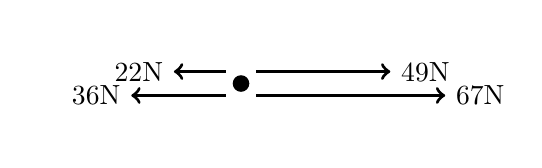
\begin{tikzpicture}
\pgfplotsset{compat=1.11}
\def\s{70} %scale
\def\FR{49} %rightward force
\def\FL{22} %leftward force
\def\FRR{67}
\def\FLL{36}
    \begin{axis}[
        width=7cm, height=3cm,
        axis line style={draw=none},
        ticks=none,
        axis lines=middle,
        ymin=-\s, ymax=\s,
        xmin=-\s, xmax=\s,
        clip=false,
    ]
    \fill (0,0) circle (3pt);
    \draw[very thick,black,->] (5,15) -- (\FR,15) node[right] {\SI{\FR}{N}};
    \draw[very thick,black,->] (5,-15) -- (\FRR,-15) node[right] {\SI{\FRR}{N}};
    \draw[very thick,black,->] (-5,15) -- (-\FL,15) node[left] {\SI{\FL}{N}};
    \draw[very thick,black,->] (-5,-15) -- (-\FLL,-15) node[left] {\SI{\FLL}{N}};
    \end{axis}
\end{tikzpicture}
\end{center}

\end{multicols}

\clearpage 

\subsection{Newton's Second Law of Motion} \label{kkBUgj}

\Gls{equilibrium} is the state when all forces on an object are balanced; the net force is zero ($\vec{F}_{\text{net}} = 0$), which implies that the object does not accelerate. A net force is also known as an unbalanced force. When a non-zero net force (e.g., $F_{\text{net}} = \SI{10}{N}$) acts on an object that's at rest, the object moves. More specifically, it accelerates: its velocity changes over a period of time.

\begin{mdframed}[backgroundcolor=black!10]
\gls{NIIL} states that the net force on an object is equal to the mass of the object multiplied by its acceleration.

\begin{equation} \label{eq:NewtonIILaw} 
    F_{\mathrm{net}} = ma
\end{equation}

\begin{center}
    \begin{tabular}{cl|cl}
    \hline
    \textbf{Symbol} & \textbf{Quantity} & \textbf{SI Base Unit} & \textbf{Unit Symbol}  \\
    \hline\hline
    \rule{0pt}{2.5ex}
        $F_{\mathrm{net}}$ & net force & newton & N\\
        $m$ & mass & kilogram & kg\\
        $a$ & acceleration & meter per second squared & \SI{}{m/s^2}\\
    \hline
    \end{tabular}
\end{center}

According to Newton's 2nd Law, net force causes acceleration. When there is a net force on an object ($\vec{F}_{\text{net}} \neq 0$), the object will accelerate in the direction of the net force.
\end{mdframed}


\begin{example} \label{ex:NetForce_Tony}
Tony pushes a 15-kg shopping cart and accelerates it by \SI{3.0}{m/s^2}. What is the net force Tony exerts on the cart?
\end{example}

\Solution We are given mass and acceleration: $m = \SI{15}{kg}$ and $a = \SI{3.0}{m/s^2}$. We want to find net force: $F_{\text{net}} =$ ? These three quantities are related by Newton's 2nd Law (Eq.~\ref{eq:NewtonIILaw}):

\begin{equation*}
    F_{\text{net}} = m a\ .
\end{equation*}

Substituting values leads to

\begin{equation*}
    F_{\text{net}} = (15)(3.0) = \SI{45}{N}.
\end{equation*}

Therefore, the net force is $\SI{45}{N}$. 

\begin{example} \label{ex:Solve_NIIL_a}
Santi pushes a lawn mower with a net force of \SI{51}{N}. The mass of the mower is \SI{24}{kg}. What is its acceleration?
\end{example}

\Solution We know net force and mass: $F_{\mathrm{net}} = \SI{51}{N}$ and $m = \SI{24}{kg}$. We want to find acceleration: $a =$ ? By Newton's 2nd Law,

\begin{equation*}
    F_{\mathrm{net}} = ma\ .
\end{equation*}

Substituting known values leads to,

\begin{equation*}
    51 = 24 a\ .
\end{equation*}

Solve this equation for acceleration by the following steps:

\begin{align*}
    \textbf{Write $a$ on left} \hspace{9cm} 
    & \hspace{-6cm} 24 a = 51\\[1ex]
    \textbf{Divide by 24} \hspace{9cm}
    & \hspace{-6cm} \frac{\cancel{24}a}{\textcolor{red}{\cancel{24}}} = \frac{51}{\textcolor{red}{24}}\\[1ex]
    \textbf{Simplify} \hspace{9cm}
    & \hspace{-6cm} a = 2.1
\end{align*}

Therefore, the acceleration of the lawn mower is  $a = \SI{2.1}{m/s^2}$.

\clearpage

\begin{example} \label{ex:TugOWar} 
Two teams play tug-of-war on a cart. One team pulls the cart leftward, and the other team pulls rightward. The net force and cart mass are shown in the free-body diagram below. What is the cart's acceleration?
\end{example}

\begin{figure}[h!]
    \centering
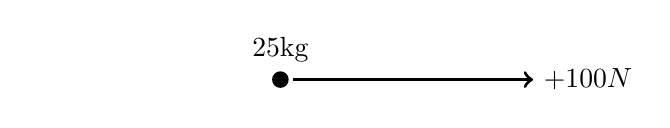
\begin{tikzpicture}
\pgfplotsset{compat=1.11}
\def\s{1}
    \begin{axis}[
        width=8cm, height=2cm,
        axis line style={draw=none},
        ticks=none,
        axis lines=middle,
        ymin=-\s, ymax=\s,
        xmin=-\s, xmax=\s,
        clip=false,
    ]
    \fill (0,0) circle (3pt) node[above=3pt] {\SI{25}{kg}};
    \draw[very thick,black,->] (0.05,0) -- (1,0) node[right] {$+\SI{100}{N}$};
    \end{axis}
\end{tikzpicture}
\end{figure}



\Solution From the free-body diagram, we know that net force is $F_{\text{net}} = \SI{100}{N}$ and mass is $m = \SI{25}{kg}$. We want to find acceleration: $a =$ ?. Here, this example proceeds like Example~\ref{ex:Solve_NIIL_a}. Newton's second law is $F_{net} = ma$, and substituting values leads to

\begin{equation*}
    100 = 25 a\ .
\end{equation*}

Solving for acceleration, as we did in Example \ref{ex:Solve_NIIL_a}, leads to

\begin{equation*}
    a = \SI{4.0}{m/s^2}\ .
\end{equation*}

\vspace{2ex}

\cyanhrule

\subsection*{\ref{kkBUgj} Exercises}

\begin{multicols}{2}

\begin{exercise} \label{01Hh51}
What is the unit of force? What is the unit symbol?
\end{exercise}

\begin{exercise} \label{YQwD8z}
One newton (N) is approximately the force on your hand from the weight of an apple. Newton's 2nd Law suggests that the newton may be equivalently expressed in terms of a the kilogram, the meter, and the second.  Using Eq.~(\ref{eq:NewtonIILaw}) to guide you, write \SI{1}{N} in terms of kg, m, and s. (\textit{Hint}: Replace the quantity symbols with their unit symbols.)
\end{exercise}

\begin{exercise} \label{aBCVA3}
Antonio pushes a 12-kg shopping cart and accelerates it by \SI{2.0}{m/s^2}. Draw the free-body diagram on the cart. What is the net force Antonio exerts on the cart?
\end{exercise}

\begin{exercise} \label{Sm9Zw6}
    If a 10-kg object accelerates at \SI{5.2}{m/s^2}, what is the net force exerted on it? Include a free-body diagram.  
\end{exercise}

\begin{exercise} \label{RbjKEg}
    A 63.0-kg sprinter starts a race with an acceleration of \SI{4.20}{m/s^2}. What is the net force on him?
\end{exercise}

\begin{exercise} \label{goj4oA}
    A cleaner pushes a 4.50-kg laundry cart with a net force of \SI{60.0}{N}. Calculate the cart's acceleration.
\end{exercise}

\begin{exercise} \label{G333de}
    The net force on a 68-kg filing cabinet is \SI{240}{N}. What is the cabinet's acceleration?
\end{exercise}

\begin{exercise} \label{8M4KDp}
    7800 newtons of net force are applied by the engine on a car to accelerate the vehicle at \SI{2.4}{m/s^2}. What is the mass of the car?
\end{exercise}

\begin{exercise} \label{EAtsO8}
    When a net force of \SI{84}{N} are exerted on an object, the object accelerates at \SI{7.0}{m/s^2}. What is the object's mass?
\end{exercise}

\begin{exercise} \label{vuAqX8}
    Solve Newton's Second Law ($F_{\text{net}} = ma$) for acceleration using no numbers, only variables. \textit{Hint}: Follow Example~\ref{ex:Solve_NIIL_a}.
\end{exercise}

\begin{exercise} \label{zVvXad}
    Solve Newton's 2nd Law for mass $m$ using only variables, no numbers.
\end{exercise}

\begin{exercise} \label{XfTcUv}
Team Red pushes a cart with a rightward force of \SI{184}{N}. Team blue pushes it with a \SI{122}{N} force to the left. The cart's mass is \SI{15.5}{kg}. (a) Draw the free-body diagram. (b) What is the cart's acceleration?
\end{exercise}

\begin{exercise} \label{uawqLb}
    Two horizontal forces on a \SI{2.0}{kg} box are \SI{13}{N} and \SI{-19}{N}. (a) Draw the free-body diagram of the box. (b) Calculate the acceleration of the box. 
\end{exercise}

\begin{exercise} \label{FWDsH3}
The object represented by the free-body diagram below accelerates at \SI{-4.0}{m/s^2}. Find the mass $m$ of the object.
\end{exercise}

\begin{figure}[h!]
    \centering
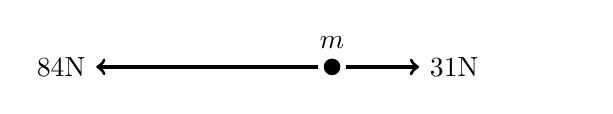
\begin{tikzpicture}
\pgfplotsset{compat=1.11}
\def\s{90}
    \begin{axis}[
        width=8cm, height=2cm,
        axis line style={draw=none},
        ticks=none,
        axis lines=middle,
        ymin=-\s, ymax=\s,
        xmin=-\s, xmax=\s,
        clip=false,
    ]
    \fill (0,0) circle (3pt) node[above=3pt] {$m$};
    \draw[very thick,black,->] (5,0) -- (31,0) node[right] {\SI{31}{N}};
    \draw[very thick,black,->] (-5,0) -- (-84,0) node[left] {\SI{84}{N}};
    \end{axis}
\end{tikzpicture}
\end{figure}


\begin{exercise} \label{GeuEOb}
What is the acceleration of the object in the free-body diagram below?
\end{exercise}

\begin{figure}[h!]
\centering
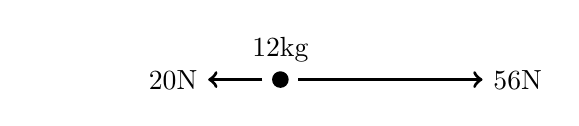
\begin{tikzpicture}
\pgfplotsset{compat=1.11}
\def\s{70}
    \begin{axis}[
        width=8cm, height=2cm,
        axis line style={draw=none},
        ticks=none,
        axis lines=middle,
        ymin=-\s, ymax=\s,
        xmin=-\s, xmax=\s,
        clip=false,
    ]
    \fill (0,0) circle (3pt) node[above=3pt]{\SI{12}{kg}};
    \draw[very thick,black,->] (5,0) -- (56,0) node[right] {\SI{56}{N}};
    \draw[very thick,black,->] (-5,0) -- (-20,0) node[left] {\SI{20}{N}};
    \end{axis}
\end{tikzpicture}
\end{figure}


\begin{exercise} \label{zaZxeE}
When horizontal forces \SI{69}{N} and \SI{-42}{N} act on a wagon, it accelerates at \SI{3.0}{m/s^2}. (a) Draw the free-body diagram. (b) What is the mass of the wagon?
\end{exercise}

\begin{exercise} \label{ejRkLz}
The external forces applied when pushing a table across the floor are shown in the free-body diagram below. (a) What is the net force on the table? (b) If the table's mass is \SI{30}{kg}, what is its acceleration? 
\end{exercise}
\vspace{-2em}

\begin{center}
\begin{tikzpicture}
\pgfplotsset{compat=1.11}
\def\s{60}
    \begin{axis}[
        width=8cm, height=4cm,
        axis line style={draw=none},
        ticks=none,
        axis lines=middle,
        ymin=-\s, ymax=\s,
        xmin=-\s, xmax=\s,
        clip=false,
    ]
    \fill (0,0) circle (3pt);
    \draw[very thick,black,->] (5,0) -- (49,0) node[right] {$F_a = \SI{49}{N}$};
    \draw[very thick,black,->] (-5,0) -- (-25,0) node[left] {$f = \SI{25}{N}$};
    \end{axis}
\end{tikzpicture}
\end{center}
\end{multicols}

\clearpage

\subsection{Friction} \label{lk8L5k}

\Gls{friction} ($f$) is an external force that acts in a direction opposite to the object's velocity. Friction is present when surfaces touch, like when a cardboard box slides across a table.

\begin{example}
When Santi (from Example~\ref{ex:Solve_NIIL_a}) accelerates a 24-kg lawn mower, he's required to push against a force of friction from the grass. This frictional force has a magnitude of \SI{30}{N}. What is the force $F_a$ that Santi needs to apply on the mower to reach a net force of \SI{51}{N}?
\end{example}

\Solution Start by drawing a free-body diagram:

\begin{figure}[h!]
\centering
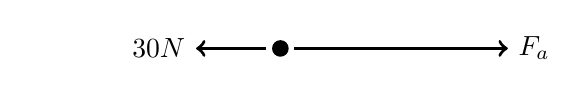
\begin{tikzpicture}
\pgfplotsset{compat=1.11}
\def\s{90}
    \begin{axis}[
        width=8cm, height=2cm,
        axis line style={draw=none},
        ticks=none,
        axis lines=middle,
        ymin=-\s, ymax=\s,
        xmin=-\s, xmax=\s,
        clip=false,
    ]
    \fill (0,0) circle (3pt);
    \draw[very thick,black,->] (5,0) -- (81,0) node[right] {$F_a$};
    \draw[very thick,black,->] (-5,0) -- (-30,0) node[left] {$\SI{30}{N}$};
    \end{axis}
\end{tikzpicture}
\end{figure}

The desired net force is

\begin{equation*}
    F_{\text{net}} = \SI{51}{N}\ ,
\end{equation*}

but from the free-body diagram net force is

\begin{equation*}
    F_{\text{net}} = F_a - 30\ .
\end{equation*}

Equating these two expressions leads to

\begin{equation*}
    F_a - 30 = 51\ .
\end{equation*}

Solve for the applied force by adding 30 to both sides:

\begin{equation*}
    F_a - 30 \mathbin{\textcolor{red}{+}} \textcolor{red}{30} 
    = 51 \mathbin{\textcolor{red}{+}} \textcolor{red}{30} = 81\ .
\end{equation*}

Therefore, Santi's applied force is

\begin{equation*}
    F_a = \SI{81}{N}\ .
\end{equation*}

\begin{example} \label{ex:SilviaCouch} 
Silvia pushes a couch across the floor. Her applied force, the frictional force, and the couch's mass are shown in the free-body diagram below. (a) What is the net force on the couch? (b) If the mass of the couch is 20-kg, what is the acceleration? 
\end{example}
\vspace{-1em}

\begin{figure}[h!]
    \centering
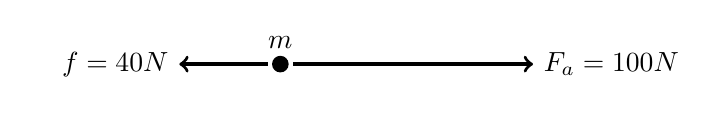
\begin{tikzpicture}
\pgfplotsset{compat=1.11}
\def\s{1}
    \begin{axis}[
        width=8cm, height=2cm,
        axis line style={draw=none},
        ticks=none,
        axis lines=middle,
        ymin=-\s, ymax=\s,
        xmin=-\s, xmax=\s,
        clip=false,
    ]
    \fill (0,0) circle (3pt) node[above=2pt] {$m$};
    \draw[very thick,black,->] (0.05,0) -- (1,0) node[right] {$F_a = \SI{100}{N}$};
    \draw[very thick,black,->] (-0.05,0) -- (-0.40,0) node[left] {$f = \SI{40}{N}$};
    \end{axis}
\end{tikzpicture}
\end{figure}


\Solution (a) From the free-body diagram, net force is applied force \textit{minus} friction (or, right \textit{minus} left):

\begin{equation*}
    F_{\text{net}} = 100 - 40 = \SI{60}{N}\ .
\end{equation*}


(b) By Newton's 2nd Law, $F_{\text{net}} = m a$, or, in this case,

\begin{equation*}
    60 = 20 a\ .
\end{equation*}

Solving for acceleration (see Example \ref{ex:Solve_NIIL_a}) leads to

\begin{equation*}
    a = \SI{3.0}{m/s^2}\ .
\end{equation*}



\begin{example} \label{ex:StalledCar} 
A 2000-kg stalled car is pushed by two people. Assume each person applies an equal force. If the car accelerates at \SI{5.0}{m/s^2} against a frictional force of \SI{300}{N}, what is the force each person applies? 
\end{example}

\Solution Start by drawing a free body diagram:

\begin{figure}[h!]
    \centering
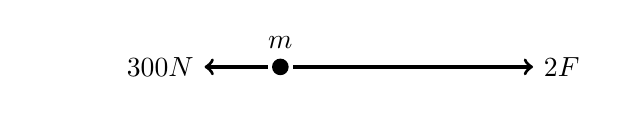
\begin{tikzpicture}
\pgfplotsset{compat=1.11}
\def\s{1}
    \begin{axis}[
        width=8cm, height=2cm,
        axis line style={draw=none},
        ticks=none,
        axis lines=middle,
        ymin=-\s, ymax=\s,
        xmin=-\s, xmax=\s,
        clip=false,
    ]
    \fill (0,0) circle (3pt) node[above=3pt] {$m$};
    \draw[very thick,black,->] (0.05,0) -- (1,0) node[right] {$2 F$};
    \draw[very thick,black,->] (-0.05,0) -- (-0.30,0) node[left] {$\SI{300}{N}$};
    \end{axis}
\end{tikzpicture}
\end{figure}


We are given values of mass, acceleration, and friction: $m = \SI{2000}{kg}$, $a = \SI{5.0}{m/s^2}$, and $f = \SI{300}{N}$. The unknown is $F$, the force applied by each person. The net force on the car, by Newton's second law, is

\begin{equation*}
    F_{\text{net}} = ma = (2000)(5.0) = \SI{10000}{N}
\end{equation*}

But net force from the free-body diagram (right \textit{minus} left; see Example \ref{ex:FnetFromFBD}) is

\begin{equation*}
    F_{\text{net}} = 2F - 300
\end{equation*}

Since the two expressions above each represent net force, we can equate them as

\begin{equation*}
    2F - 300 = \SI{10000}{}
\end{equation*}

This equation is solved for $F$ as follows:

\begin{align*}
    \textbf{Add 300} \hspace{9cm} 
    & \hspace{-6cm} 2F - 300 \mathbin{\textcolor{red}{+}} \textcolor{red}{300} = \SI{10000}{} \mathbin{\textcolor{red}{+}} \textcolor{red}{300}\\[1ex]
    \textbf{Simplify} \hspace{9cm}
    & \hspace{-6cm} 2F = \SI{10300}{}\\[1ex]
    \textbf{Divide by 2} \hspace{9cm}
    & \hspace{-6cm} \frac{\cancel{2}F}{\textcolor{red}{\cancel{2}}} = \frac{\SI{10300}{}}{\textcolor{red}{2}}\\[1ex]
    \textbf{Simplify} \hspace{9cm} 
    & \hspace{-6cm} F = 5150
\end{align*}

Therefore, the force each person applies on the car is \SI{5150}{N}.
\vspace{2ex}

\cyanhrule

\subsection*{\ref{lk8L5k} Exercises}

\begin{multicols}{2}

\begin{exercise} \label{lqMcA5}
The net force on a shopping cart is \SI{76}{N}. The person pushing the cart pushes against a frictional force of \SI{12}{N}. (a) Draw the free-body diagram showing the frictional and applied forces. (b) What is the person's applied force?
\end{exercise}

\begin{exercise} \label{Og290b}
The net force on an object is $\vec{F}_{\text{net}} = \SI{-25}{N}$. If the applied force is \SI{-46}{N}, what is the frictional force? 
\end{exercise}

\begin{center}
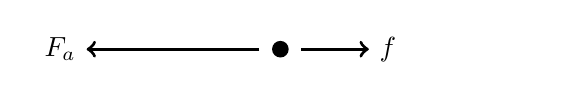
\begin{tikzpicture}
\pgfplotsset{compat=1.11}
\def\s{60}
    \begin{axis}[
        width=8cm, height=2cm,
        axis line style={draw=none},
        ticks=none,
        axis lines=middle,
        ymin=-\s, ymax=\s,
        xmin=-\s, xmax=\s,
        clip=false,
    ]
    \fill (0,0) circle (3pt);
    \draw[very thick,black,->] (5,0) -- (21,0) node[right] {$f$};
    \draw[very thick,black,->] (-5,0) -- (-46,0) node[left] {$F_a$};
    \end{axis}
\end{tikzpicture}
\end{center}

\begin{exercise} \label{naDHpo}
A 1965-kg stalled car is pushed by two people. Assume each person applies an equal force. If the car accelerates at \SI{3.5}{m/s^2} against a frictional force of \SI{480}{N}, what is the force each person applies? 
\end{exercise}

\begin{exercise} \label{w6N0j0}
14 people push an 8100-kg bus to get it started. An acceleration of at least \SI{7.0}{m/s^2} is required to start the bus, and friction between the bus and the road is \SI{900}{N}. Assuming each individual applies the same force, what is the magnitude of this individual force?
\end{exercise}

\begin{exercise} \label{WHMhQG}
    What is the answer to Example~\ref{ex:StalledCar} if there were five people pushing instead of two? Assume each person applies the same force and all other things being equal.
\end{exercise}

\begin{exercise} \label{DV094w}
Four \href{https://en.wikipedia.org/wiki/Spacecraft_propulsion#/media/File:Shuttle_Main_Engine_Test_Firing.jpg}{thrusters} propel a 2100-kg jet forward though the atmosphere against \SI{650}{N} of air resistance. If the jet accelerates at \SI{49}{m/s^2}, what is the force applied be each thruster? 
\end{exercise}

\begin{exercise} \label{e1ANRE}
Solve Example \ref{ex:StalledCar} for $F$ generally (without any numbers) using only the variables $f$, $m$, $a$, and $n$, where $n$ is the number of equal forces exerted on the object.
\end{exercise}

\end{multicols}

\clearpage

\subsection{Weight} \label{CWxEgd}

So far, we have seen only horizontal forces. Forces also apply in vertical directions. See the following.

\begin{example} \label{ex:weightIntro} 
A bowling ball is dropped from rest from the top of a cliff. (a) What is the ball's acceleration? (\textit{Hint}: Recall Unit 3: Projectiles.) (b) If the ball's mass is \SI{5}{kg}, what is the net force on it?
\end{example}

\Solution

\begin{center}
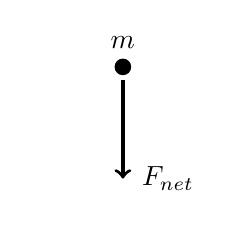
\begin{tikzpicture}
\pgfplotsset{compat=1.11}
\def\s{10}
    \begin{axis}[
        width=4cm, height=3cm,
        axis line style={draw=none},
        ticks=none,
        axis lines=middle,
        ymin=-\s, ymax=0,
        xmin=-\s, xmax=\s,
        clip=false,
    ]
    \fill (0,0) circle (3pt) node[above=3pt] {$m$};
    \draw[very thick,black,->] (0,-1.2) -- (0,-10) node[right=3pt] {$F_{\text{net}}$};
    \end{axis}
\end{tikzpicture}
\end{center}

(a) As discussed in the previous unit, the object accelerates downward due to gravity at a rate of 

\begin{equation*}
    a = -g = -\SI{9.8}{m/s^2}\ .
\end{equation*}

(b) By Newton's 2nd law (Eq.~\ref{eq:NewtonIILaw}), the net force is

\begin{equation*}
    \vec{F}_{\text{net}} = m a = -m g = -(5)(9.8) = -\SI{49}{N}\ .
\end{equation*}

Therefore, the force of gravity on the bowling ball is \SI{49}{N} downward. This result---that the magnitude of the force of gravity on an object is $mg$---is important, because this force is always present on the object, whether the object is in free-fall or not. We call it weight.

\begin{mdframed}[backgroundcolor=black!10]
\Gls{weight} ($w$) is the downward force of gravity on an object of mass $m$:

\begin{equation} \label{eq:weight} 
    w = mg
\end{equation}

\begin{center}
    \begin{tabular}{cl|cl}
    \hline
    \textbf{Symbol} & \textbf{Quantity} & \textbf{SI Base Unit} & \textbf{Unit Symbol}  \\
    \hline\hline
    \rule{0pt}{2.5ex}
        $w$ & weight & newton & N\\
        $m$ & mass & kilogram & kg\\
        $g$ & acceleration due to gravity & meter per second squared & \SI{}{m/s^2}\\
    \hline
    \end{tabular}
\end{center}

Gravitational acceleration is $g = \SI{9.8}{m/s^2}$. It's no surprise that the equation for weight (Eq.~\ref{eq:weight}) looks like Newton's Second Law (Eq.~\ref{eq:NewtonIILaw}), as we use the latter in Example~\ref{ex:weightIntro} to derive the former. 
\end{mdframed}

\cyanhrule

\subsection*{\ref{CWxEgd} Exercises}

\begin{multicols}{2}
\begin{exercise}
Compare weight and mass. (a) What are the units of weight? (b) What are the units of mass? (c) Are mass and weight the same thing? (d) Which is always constant? and which may change? (\textit{Hint}: Astronauts in space are said to be ``\href{https://youtu.be/C3GC5LS6e6Q}{weightless}.'')
\end{exercise}

\begin{exercise} \label{eStk9M}
What is the weight of a box with a mass of \SI{10}{kg}?
\end{exercise}

\begin{exercise} \label{x9Ufbz}
A 44-kilogram person has a weight of \rule{1cm}{0.15mm} newtons.
\end{exercise}

\begin{exercise} \label{r7dwXZ}
An adult grizzly bear can ``weigh'' up to \SI{300}{kg}---that's actually its \textit{mass}. What is the weight of the bear, in newtons, as we have defined it above?
\end{exercise}

\begin{exercise} \label{neLJbr}
What is the mass of a dumbbell whose weight is \SI{2450}{N}? (\textit{Hint}: Review the solution to Example~\ref{ex:Solve_NIIL_a}.)
\end{exercise}
\end{multicols}


\clearpage

\subsection{Newton's Third Law of Motion} \label{N3R3iq}

\begin{mdframed}[backgroundcolor=black!10]
\Gls{NIIIL} states that when one object exerts a force on a second object, the first object experiences a force that is equal in magnitude and opposite in direction to the force that it exerts.
\end{mdframed}

An application of Newton's Third Law is the \gls{normal force} ($F_{\text{N}}$), which is the force that a surface applies to an object. For example, the normal force is the upward force that a table exerts on a book to support the book's weight.

\begin{example} \label{A8Qdlc}
Consider a box with a mass of \SI{7}{kg} at rest on a table. What is the magnitude of the normal force on the box? 
\end{example}

\Solution The box's weight, by Eq.~(\ref{eq:weight}), is

\begin{equation*}
    w = m g = (7)(9.8) = \SI{68.6}{N}\ .
\end{equation*}

Through its weight, the box applies a downward force of \SI{68.6}{N} on the table. Since the box is not moving, all forces on it must be balanced ($F_{\text{net}} = 0$). In other words, the box is in equilibrium. To maintain this equilibrium, the table must exert, according to Newton's Third Law, a force that is equal to the box's weight (\SI{68.6}{N}) but in the upward direction. We call this force the normal force.

\begin{center}
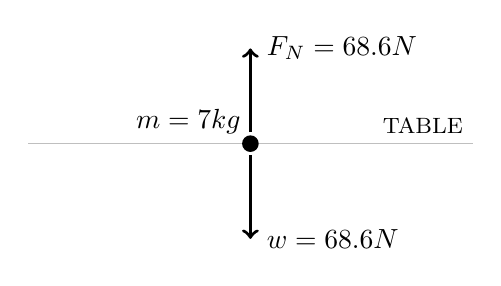
\begin{tikzpicture}
\pgfplotsset{compat=1.11}
\def\s{10}
    \begin{axis}[
        width=4cm, height=4cm,
        axis line style={draw=none},
        ticks=none,
        axis lines=middle,
        ymin=-\s, ymax=\s,
        xmin=-15, xmax=15,
        clip=false,
    ]
    \draw[lightgray] (-35,0) -- (35,0) node[above left,black] {\footnotesize TABLE}; 
    \fill (0,0) circle (3pt) node[above left] {$m = \SI{7}{kg}$};
    \draw[very thick,black,->] (0,+1.2) -- (0,+10) node[right=2pt] {$F_{\text{N}} = \SI{68.6}{N}$};
    \draw[very thick,black,->] (0,-1.2) -- (0,-10) node[right=2pt] {$w = \SI{68.6}{N}$};
    \end{axis}
\end{tikzpicture}
\end{center}


\cyanhrule

\subsection*{\ref{N3R3iq} Exercises}

\begin{multicols}{2}

\begin{exercise} \label{f03y7Z}
    Suppose you are installing a smoke detector in the ceiling of your house. You push up on the detector to snap it into place. What is the direction of the normal force exerted by the ceiling on the detector?
\end{exercise}

\begin{exercise} \label{BkOxdJ}
Judy, whose mass is \SI{60}{kg}, lays down on a park bench. What is the normal force by the bench on Judy?
\end{exercise}


\begin{exercise} \label{QaZUiq}
What is the magnitude and direction of the normal force on a \SI{100}{kg} container at rest on a table?
\end{exercise}

\begin{exercise} \label{wkga6W}
Consider the \SI{7}{kg} box from Example \ref{A8Qdlc}. (a) Re-draw the free-body diagram to show a person pushing down on the box with a force of \SI{84}{N}. (b) What is the normal force on the box now?
\end{exercise}

\begin{exercise} \label{hIgPqQ}
Ben, the 80-kilogram zookeeper is standing on a platform at the zoo. (a) Draw a free-body diagram including Ben's weight and the normal force on him. (b) What is the magnitude of the normal force on Ben? (c) If he picks up a container of water weighing \SI{215}{N}, what is the normal force exerted by the platform now? 
\end{exercise}

\begin{exercise} \label{SwLQsz}
    Bob is at the gym. He sees a \SI{65}{kg} dumbbell at rest on a rack and tries to pick it up, but he applies only a 500-newton upward force on the weight. (a) Draw a free-body diagram of Bob's feeble attempt to lift the weight. (b) The instant the upward force is exerted, what is the normal force of the rack on the dumbbell?
\end{exercise}

\end{multicols}



% \clearpage

% \textbf{Review Problems}

% \begin{exercise}
% Calculate the net force from the free-body diagram below.
% \vspace{-0.8em}

% \begin{center}
% \begin{tikzpicture}
% \pgfplotsset{compat=1.11}
% \begin{axis}[
%     width=8cm,height=2cm,
%     axis line style={draw=none},
%     ticks=none,
%     xmin=-10,xmax=10,
%     ymin=-10,ymax=10,
%     clip=false,
% ]
%     \fill (0,0) circle (2pt);
%     \draw[thick,->] (0.5,0) -- (5.4,0) node[right] {\SI{54}{N}};
%     \draw[thick,->] (-0.5,0) -- (-4.9,0) node[left] {\SI{49}{N}};
% \end{axis}  
% \end{tikzpicture}
% \end{center}
% \end{exercise}

% \begin{exercise}
% The sprinter Jessica, whose mass is 41.0-kg, starts a race with an acceleration of \SI{3.93}{m/s^2}. What is the net force on her?
% \iflong
% {\color{red} Answer: \SI{161}{N}}
% \else \fi
% \end{exercise}

% \begin{exercise}
% If a net force of \SI{21000}{N} is exerted on a 750-kg vehicle, what is the vehicle's acceleration?
% \iflong
% {\color{red} Answer: \SI{28}{m/s^2}}
% \else \fi
% \end{exercise}

% \begin{exercise}
%     The net force on an object accelerating at \SI{8.0}{m/s^2} is \SI{256}{N}. What is the object's mass?
%     \iflong
%     {\color{red} Ans: \SI{32}{kg}}
%     \else \fi
% \end{exercise}

\clearpage
\printnoidxglossaries

\clearpage
\subsection{Answers to Select Exercises}

\begin{multicols}{2}
\ref{WTFwXI}. (a) No, because the cart will not stay in motion if it is acted on by a net force. (b) A net force supplied by friction between the floor and wheels.\\
\ref{MB3Xar} (a) Since the bear has more mass, it has more inertia. (b) The bear will have a greater tendency than you to stay in motion \textit{in a straight line}; it's less able to do zig-zag motions.\\
\ref{RApeJt}. $+\SI{100}{N}$\\
\ref{MUJe54}. $-\SI{50}{N}$\\
\ref{Uhrg0I}. \SI{0}{N}\\
\ref{Wu1JXi}. $+\SI{38}{N}$\\
\ref{Tj5icu}. $-\SI{38}{N}$\\
\ref{nMwKjy}. \SI{0}{N}\\
\ref{Js7KjP}. $+\SI{58}{N}$\\
\ref{01Hh51}. newton (N)\\
\ref{YQwD8z}. $\SI{1}{N} \equiv \SI{1}{kg} \cdot \SI{1}{m/s^2}$\\
\ref{aBCVA3}. \SI{24}{N}\\
\ref{Sm9Zw6}. \SI{52}{N}\\
\ref{RbjKEg}. \SI{265}{N}\\
\ref{goj4oA}. \SI{13.3}{m/s^2}\\
\ref{G333de}. \SI{3.53}{m/s^2}\\
\ref{8M4KDp}. \SI{3250}{kg}\\
\ref{EAtsO8}. \SI{12}{kg}\\
\ref{vuAqX8}. $a = \frac{F_{\text{net}}}{m}$\\
\ref{zVvXad}. $m = \frac{F_{\text{net}}}{a}$\\
\ref{XfTcUv}. (b) \SI{4.0}{m/s^2}\\
\ref{uawqLb}. \SI{-3.0}{m/s^2}\\
\ref{FWDsH3}. \SI{13}{kg}\\
\ref{GeuEOb}. \SI{3.0}{m/s^2}\\
\ref{zaZxeE}. \SI{9.0}{kg}\\
\ref{ejRkLz}. \SI{0.8}{m/s^2}\\
\ref{lqMcA5}. \SI{64}{N}\\
\ref{Og290b}. $+\SI{21}{N}$\\
\ref{naDHpo}. \SI{3679}{N}\\
\ref{w6N0j0}. \SI{4114}{N}\\
\ref{WHMhQG}. \SI{2060}{N}\\
\ref{DV094w}. \SI{25888}{N}\\
\ref{e1ANRE}. $F = \frac{ma + f}{n}$\\
\ref{eStk9M}. \SI{98}{N}\\
\ref{x9Ufbz}. \SI{431.2}{N}\\
\ref{r7dwXZ}. \SI{2940}{N}\\
\ref{neLJbr}. \SI{250}{kg}\\
\ref{f03y7Z}. Down\\
\ref{BkOxdJ}. \SI{588}{N}\\
\ref{QaZUiq}. \SI{980}{N}\\
\ref{wkga6W}. \SI{152.6}{N}\\
\ref{hIgPqQ}. (b) \SI{784}{N} \hspace{1em} (c) \SI{999}{N}\\
\ref{SwLQsz}. (b) \SI{137}{N}\\


\end{multicols}

\end{document}